\section{现状:产品力强大,链接企业内外}

\subsection{财务状况:订阅收入为主,non-GAAP稳定盈利}

\textbf{Atlassian 的收入主要来自订阅收入、永久许可、维修收入和其他来源}。其中:
\begin{enumerate}
    \item 订阅是 Atlassian 收入的主要来源,占比逐年提高,1Q23占总收入的 80\%。订阅收入主要由活跃许可证的数量和大小、产品类型和许可证的价格驱动,预计未来受益于云计算进一步普及仍将持续增加。
    \item 永久许可证收入包括从向新客户销售许可证、增加现有客户中的用户数量和向现有客户增加许可证中确认的收入。2021年Atlassian取消了永久许可证业务,鼓励用户转向云订阅。
    \item 维护收入是指为永久许可产品向客户支持所获得的费用,但受永久许可证不再签发影响有所萎缩。
    \item 其他收入包括在 Atlassian Marketplace销售第三方应用程序和培训服务的费用。Atlassian Marketplace类似App Store,在第三方销售收入中抽成比例为15-25\%。这部分收入随Atlassian生态的逐步完善吸引更多第三方应用开发者,增长也非常迅速,但体量较小。
\end{enumerate}
\begin{figure}[H]
    \caption{Atlassian分业务收入(万美元)}
    \begin{center}
        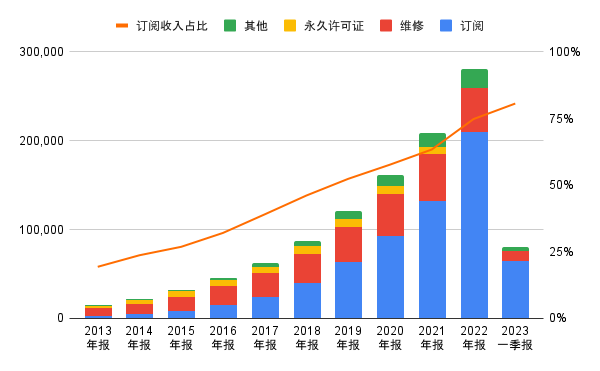
\includegraphics[width=\linewidth]{img/revenue.png}
    \end{center}
    \footnotesize{资料来源:同花顺iFind}
\end{figure}

\textbf{费用上,Atlassian轻营销、重研发}。一般的SaaS和软件厂商由于大量的营销费用呈现出高毛利、低净利的情况。Atlassian采用直销的方式降低营销成本,并且拳头产品的口碑非常好,一度不需要销售人员。Atlassian 销售费用率始终低于研发费用率,销售费用率常年在 20\%上下浮动(正常的 SAAS 企业销售费用率在40\%-60\%,个别企业甚至在 80\%左右)。此外Atlassian重研发,研发费用率接近50\%,不断研发新功能以贴合软件行业的快速发展。近期Atlassian将挑战性的宏观经济环境视为抢占市场份额并继续投资于战略性高增长领域的机会,费用率均有所增加。

\begin{figure}[H]
    \caption{Atlassian费用水平(万美元)}
    \begin{center}
        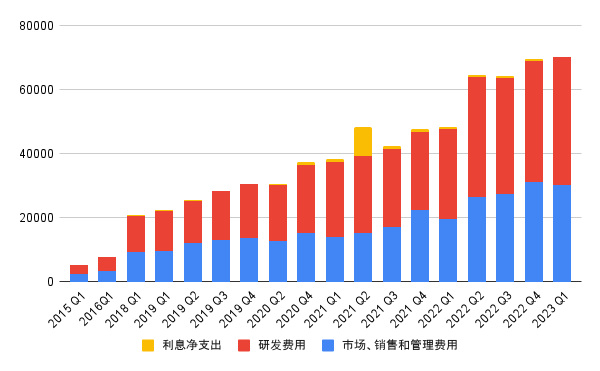
\includegraphics[width=0.9\linewidth]{img/cost.png}
    \end{center}
    \footnotesize{资料来源:同花顺iFind}
\end{figure}
\begin{figure}[H]
    \caption{同行业其他公司的销售费用率对比}
    \begin{center}
        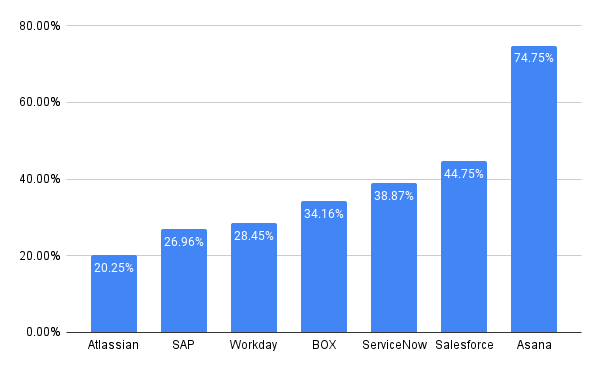
\includegraphics[width=0.9\linewidth]{img/SM.png}
    \end{center}
    \footnotesize{资料来源:同花顺iFind}
\end{figure}

\textbf{Atlassian保持长期盈利,non-GAAP净利持续为正}。Atlassian在未上市时便保持了长期的盈利,上市后营业利润率保持增长趋势,但2022年由于公司扩张战略、叠加高通胀的宏观环境,公司的营业利润率有所下滑。
\begin{figure}[H]
    \caption{non-GAAP口径下Atlassian财务状况}
    \begin{center}
        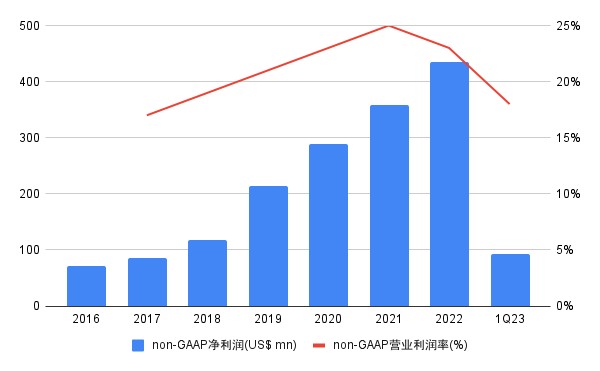
\includegraphics[width=\linewidth]{img/non-GAAP.png}
    \end{center}
    \footnotesize{资料来源:公司公告}
\end{figure}

\subsection{产品线:覆盖软件开发流程,链接需求、开发团队与业务团队}
Atlassian的产品线主要有以下几条:协助团队敏捷开发、DevOps的 Jira Software(以下简称为Jira)和Bitbucket等、用于工作协同的 Confluence和Trello等、用于IT服务的Jira Service Management。Atlassian新推出了Atlassian Together订阅套餐,包括了Tello、Confluence、Jira产品等。

\textbf{Jira等一系列应用在敏捷开发时代为软件开发组织提供了工作流}。互联网行业的快速发展使得敏捷开发快速响应需求的重要性大大提升,但组织、代码和事务的复杂度严重拖累了敏捷响应的速度。Atlassian提供了一整套全流程的敏捷开发与DevOps解决方案以对抗复杂度:核心产品Jira具有规划、跟踪、发布、报告和自动化五大用途,将事务与代码关联起来,可以规划分配大型任务,并提供了许多标准工作流辅助开发;与Jira高度集成的代码托管网站Bitbucket则覆盖了代码的编写、审查和CI/CD;Atlassian旗下的另一款软件Opsgene则集中管理警报,在业务逻辑发生问题时及时通知给正确的人,也与Jira高度集成;Statuspage则负责监控软件的日常运行。Jira自发布以来广受赞誉,以Jira为核心的软件开发全流程覆盖是Atlassian的核心竞争力之一。
\begin{figure}[H]
    \caption{Jira依旧是使用最多的敏捷开发工具}
    \begin{center}
        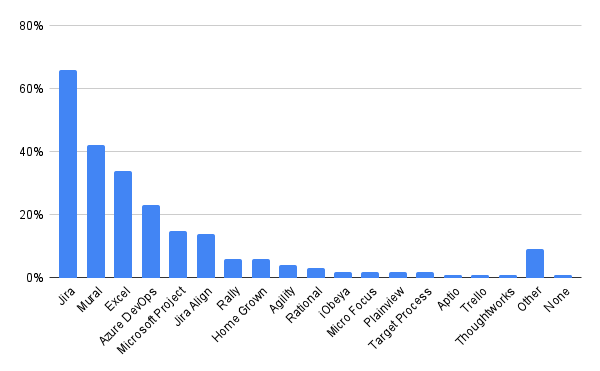
\includegraphics[width=\linewidth]{img/popularity.png}
    \end{center}
    \footnotesize{资料来源:digital.ai。注:digital.ai的Agility为Jira竞品}
\end{figure}
\begin{table}[H]
    \caption{Jira Software 五大用途}
    \begin{tabular}{ll}
        \toprule
        用途  & 内容                             \\
        \midrule
        规划  & 通过用户故事、事务和任务,将宏大计划分解为易于管理的部分   \\
        跟踪  & 追踪bug与需求,排定整个环境中团队工作的优先次序并进行讨论 \\
        发布  & 加速交付,同时保证自己所拥有的信息保持最新          \\
        报告  & 根据直观的实时数据,在整体环境下提升团队绩效         \\
        自动化 & 通过无代码自动化功能,节省时间、保持专注、顺畅工作流     \\
        \bottomrule
    \end{tabular}
    \footnotesize{资料来源:Atlassian}
\end{table}

\textbf{工作协同方面,Confluence实现企业内部的知识共享,Trello专注于通用的任务管理}。Confluence是一个社会性的、灵活的内容协作平台,用于创建、共享、组织和讨论项目。不同于一般的协作文档,Confluence针对技术团队提供了大量的规范模版,并支持富媒体编辑,满足技术文档中的UML类图、Visio图、流程图的需求;文档中还可以内嵌评审流程,不止于仅仅@某人,关联研发过程。通过软件开发者中的盛誉,Confluence也向企业技术人员、知识工作者等群体破圈传播。相较于Jira所包含的以敏捷开发一个软件产品为目标的任务管理,Trello则提供了更通用的看板,提供了任务进度等要素,帮助团队对任务进行计划。
\begin{figure}[H]
    \begin{minipage}{0.48\linewidth}
        \caption{Jira任务管理基于产品目标}
        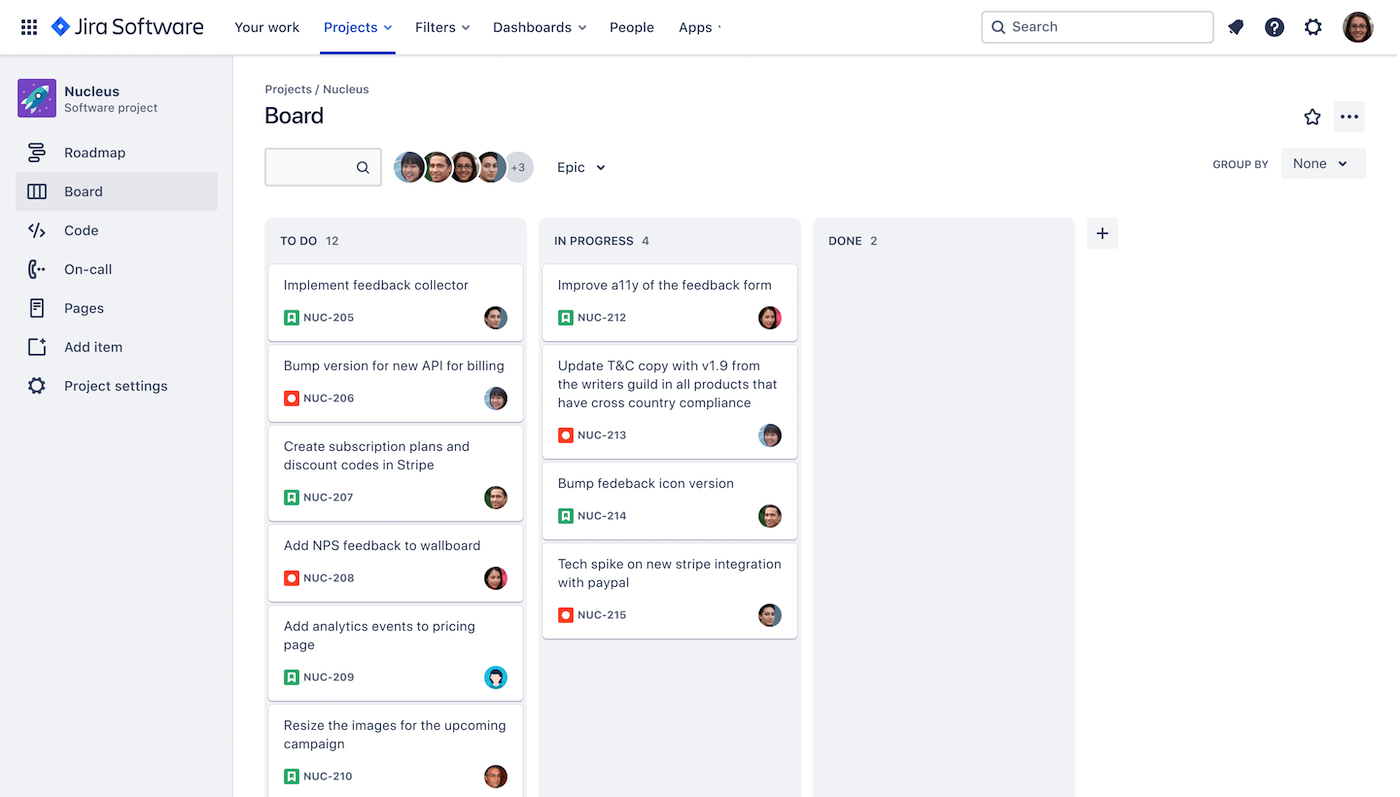
\includegraphics[width=\linewidth]{img/jira.png}
    \end{minipage}
    \begin{minipage}{0.48\linewidth}
        \caption{Trello任务管理更为通用}
        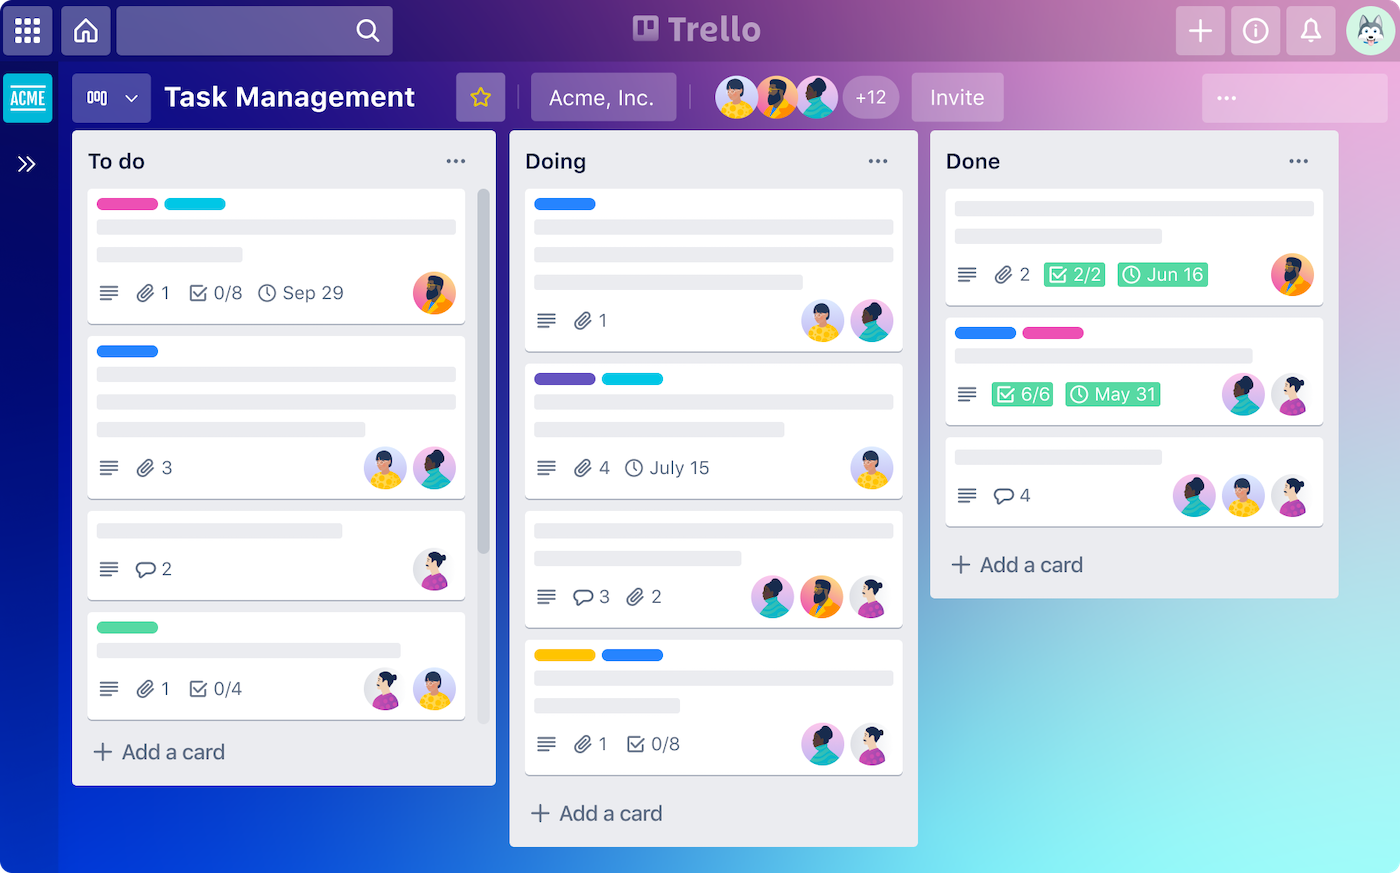
\includegraphics[width=\linewidth]{img/Trello.png}
    \end{minipage}

    \footnotesize{资料来源:technologyadvice}
\end{figure}

\textbf{IT服务管理(ITSM)方面,Jira Service Management(JSM)连接开发、IT 运营和业务团队}。企业提供技术服务的瓶颈并不只是技术层面,流程管理与人员疏失的失误可能会导致IT服务的失败,因而需要ITSM以保证IT服务质量,协作不应当局限在开发团队而是所有团队,所以Atlassian推出了JSM。JSM可以作为自助服务门户,为用户提供了一个可以寻求帮助的地方。客户需要服务时可以向JSM请求帮助,企业内部可以履行或通过ITSM移交服务请求给其他适当团队,如IT、人力、法律和财务团队等。Jira Service Management在 Jira 之上提供专业的 ITSM 功能,将开发、运营和业务团队汇聚在一起,以便他们可以及时响应业务变更并快速提供出色的服务体验,目前市占率(18.5\%)排行第二,仅次于ServiceNow(40.1\%)。
\begin{figure}[H]
    \caption{JSM功能}
    \begin{center}
        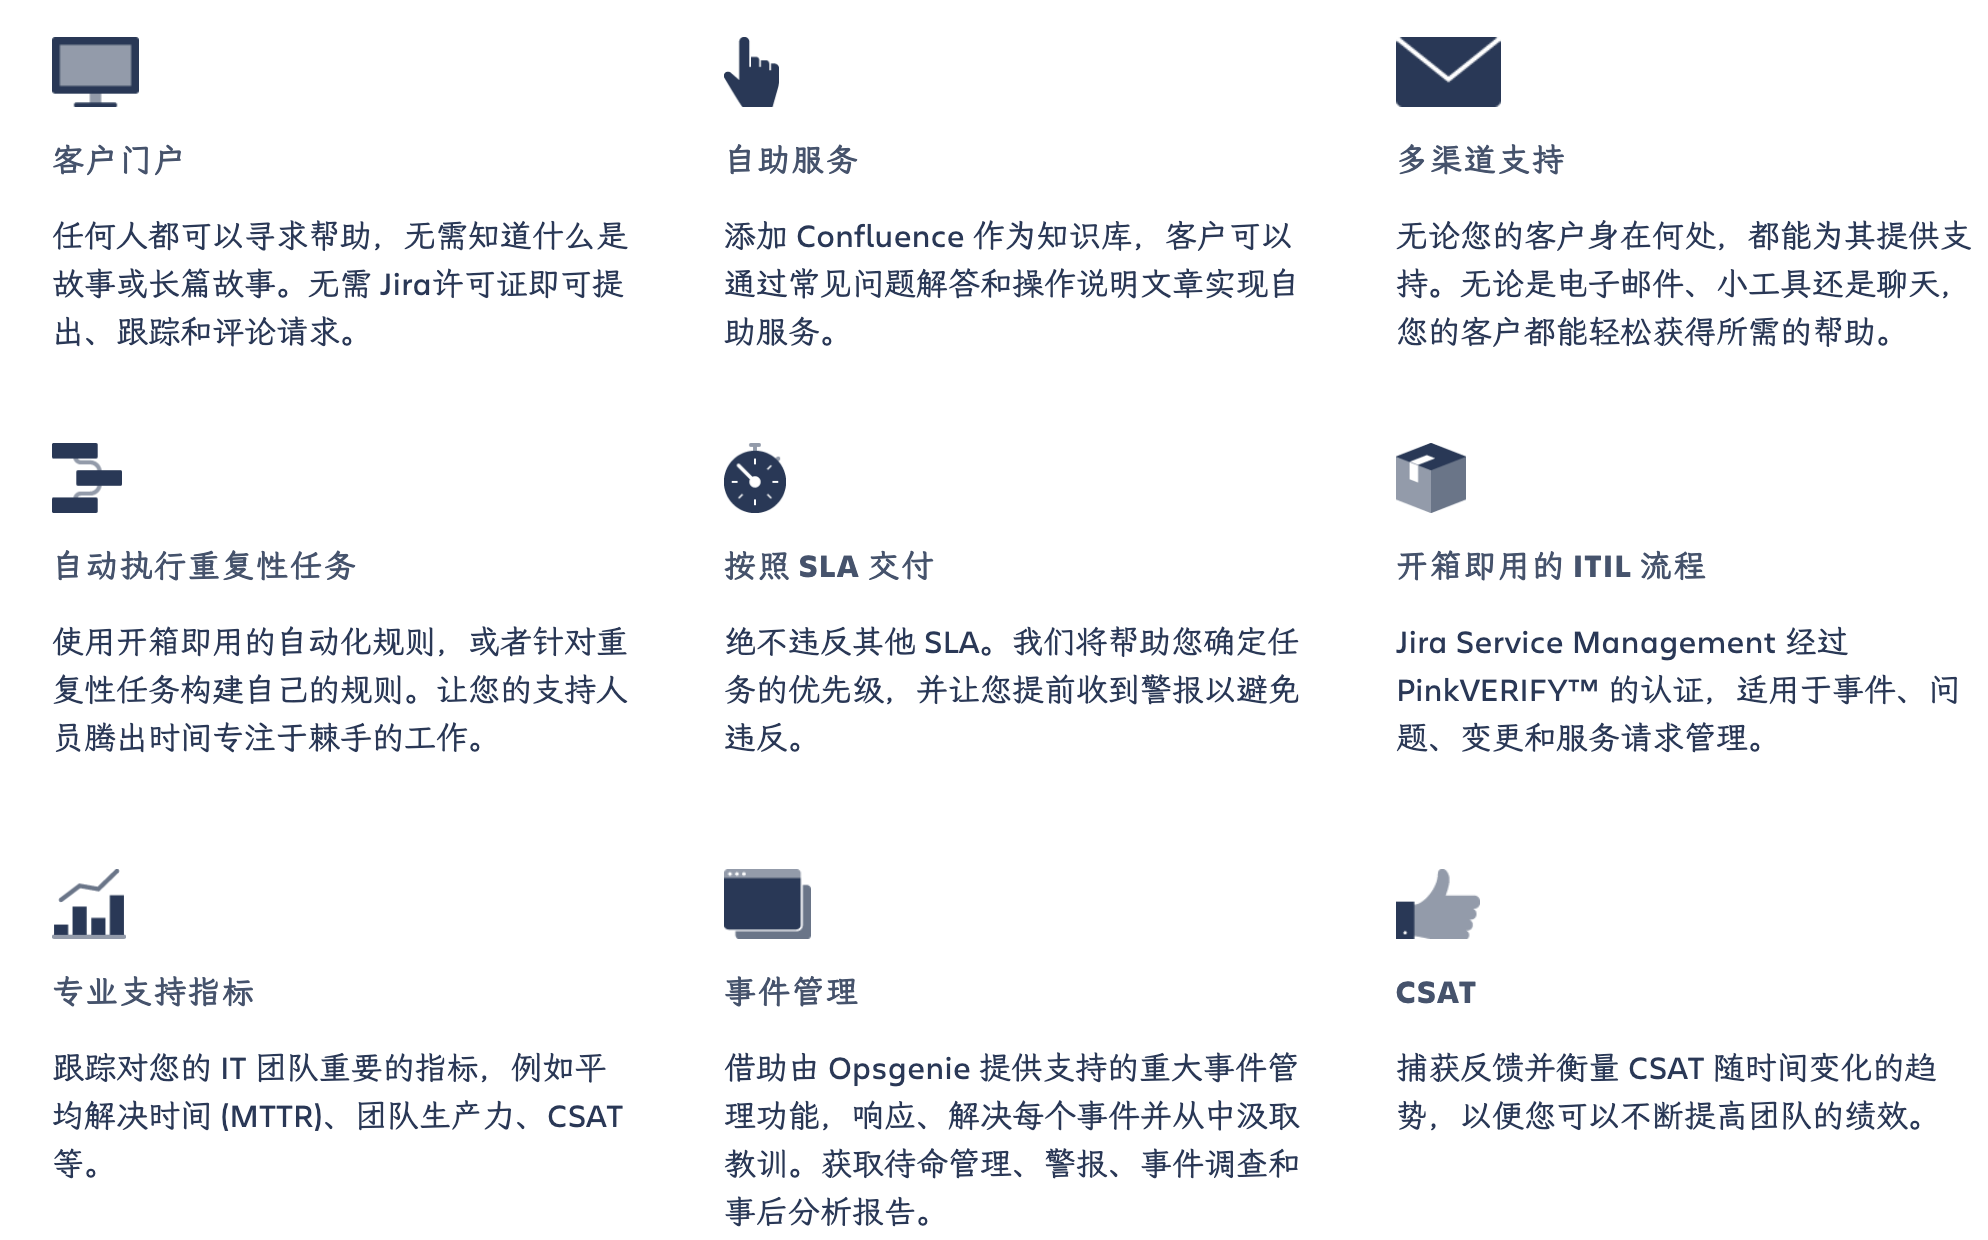
\includegraphics[width=0.9\linewidth]{img/ITSM.png}
    \end{center}
    \footnotesize{资料来源:atlassian}
\end{figure}

\subsection{行业:百舸争流,角逐激烈}

目前Atlassian在三个产品领域均有竞争对手,但市场空间相对广阔。根据\href{https://startuptalky.com/atlassian-success-story/}{startuptalky},2021 年,项目管理软件市场产生了 53.596 亿美元的销售额。到 2032 年,项目管理软件市场的收入预计将达到 204亿美元,2022 年至 2032 年的复合年增长率为 13.1\%。与之相对Atlassian年化收入仅16亿美元。且Atlassian凭借∆强大的产品力具有一定的竞争优势。

开发工具方面,据enlyft,Jira市场份额约为28.95\%。其主要竞争对手包括微软(Azure Board与GitHub Enterprise)、GitLab、IBM、Broadcom(Rally)、Asana、JetBrains(YouTrack)等。据Gartner,Jira为最受欢迎的敏捷开发工具,相较于其他产品服务更加完善、更易部署、价格相对便宜。

工作协同领域竞争较为激烈。据enlyft,文档工具领域Confluence市场份额约为2.25\%,任务管理领域Trello占统治性地位,市占率达74.1\%。Atlassian在这些方面的主要竞争对手包括微软Office、Slack、Adobe、Google Workspace、Notion等,在技术文档的细分领域Confluence凭借富媒体、易集成等具有一定的比较优势。

ITSM方面,其主要竞争对手包括ServiceNow、GoTo、微软等,JSM在ITSM市占率仅次于ServiceNow,达18.5\%。
\begin{figure}[H]
    \caption{JSM在ITSM领域市占率排第二}
    \begin{center}
        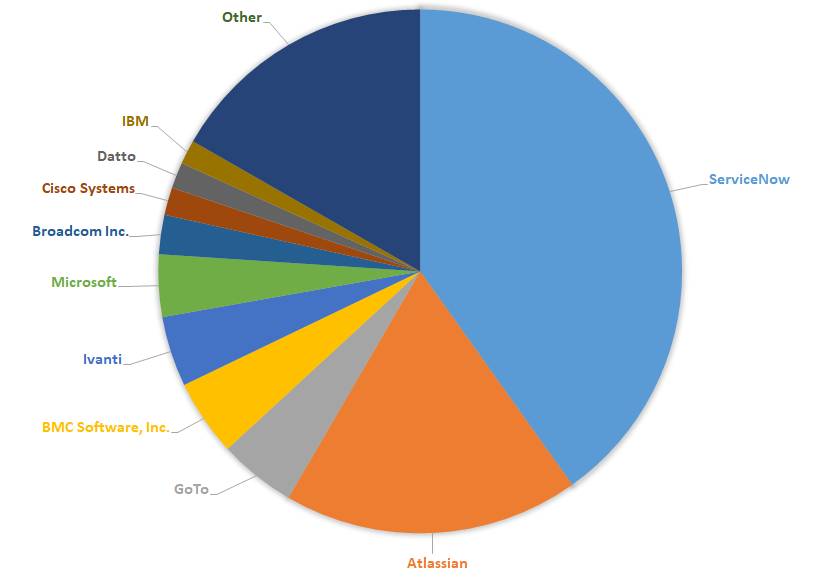
\includegraphics[width=0.9\linewidth]{img/JSM.png}
    \end{center}
    \footnotesize{资料来源:Apps Run The World}
\end{figure}
